\documentclass[twoside]{book}

% Packages required by doxygen
\usepackage{fixltx2e}
\usepackage{calc}
\usepackage{doxygen}
\usepackage[export]{adjustbox} % also loads graphicx
\usepackage{graphicx}
\usepackage[utf8]{inputenc}
\usepackage{makeidx}
\usepackage{multicol}
\usepackage{multirow}
\PassOptionsToPackage{warn}{textcomp}
\usepackage{textcomp}
\usepackage[nointegrals]{wasysym}
\usepackage[table]{xcolor}

% Font selection
\usepackage[T1]{fontenc}
\usepackage[scaled=.90]{helvet}
\usepackage{courier}
\usepackage{amssymb}
\usepackage{sectsty}
\renewcommand{\familydefault}{\sfdefault}
\allsectionsfont{%
  \fontseries{bc}\selectfont%
  \color{darkgray}%
}
\renewcommand{\DoxyLabelFont}{%
  \fontseries{bc}\selectfont%
  \color{darkgray}%
}
\newcommand{\+}{\discretionary{\mbox{\scriptsize$\hookleftarrow$}}{}{}}

% Page & text layout
\usepackage{geometry}
\geometry{%
  a4paper,%
  top=2.5cm,%
  bottom=2.5cm,%
  left=2.5cm,%
  right=2.5cm%
}
\tolerance=750
\hfuzz=15pt
\hbadness=750
\setlength{\emergencystretch}{15pt}
\setlength{\parindent}{0cm}
\setlength{\parskip}{0.2cm}
\makeatletter
\renewcommand{\paragraph}{%
  \@startsection{paragraph}{4}{0ex}{-1.0ex}{1.0ex}{%
    \normalfont\normalsize\bfseries\SS@parafont%
  }%
}
\renewcommand{\subparagraph}{%
  \@startsection{subparagraph}{5}{0ex}{-1.0ex}{1.0ex}{%
    \normalfont\normalsize\bfseries\SS@subparafont%
  }%
}
\makeatother

% Headers & footers
\usepackage{fancyhdr}
\pagestyle{fancyplain}
\fancyhead[LE]{\fancyplain{}{\bfseries\thepage}}
\fancyhead[CE]{\fancyplain{}{}}
\fancyhead[RE]{\fancyplain{}{\bfseries\leftmark}}
\fancyhead[LO]{\fancyplain{}{\bfseries\rightmark}}
\fancyhead[CO]{\fancyplain{}{}}
\fancyhead[RO]{\fancyplain{}{\bfseries\thepage}}
\fancyfoot[LE]{\fancyplain{}{}}
\fancyfoot[CE]{\fancyplain{}{}}
\fancyfoot[RE]{\fancyplain{}{\bfseries\scriptsize Generated on Thu Jun 4 2015 16\+:15\+:23 for My Project by Doxygen }}
\fancyfoot[LO]{\fancyplain{}{\bfseries\scriptsize Generated on Thu Jun 4 2015 16\+:15\+:23 for My Project by Doxygen }}
\fancyfoot[CO]{\fancyplain{}{}}
\fancyfoot[RO]{\fancyplain{}{}}
\renewcommand{\footrulewidth}{0.4pt}
\renewcommand{\chaptermark}[1]{%
  \markboth{#1}{}%
}
\renewcommand{\sectionmark}[1]{%
  \markright{\thesection\ #1}%
}

% Indices & bibliography
\usepackage{natbib}
\usepackage[titles]{tocloft}
\setcounter{tocdepth}{3}
\setcounter{secnumdepth}{5}
\makeindex

% Hyperlinks (required, but should be loaded last)
\usepackage{ifpdf}
\ifpdf
  \usepackage[pdftex,pagebackref=true]{hyperref}
\else
  \usepackage[ps2pdf,pagebackref=true]{hyperref}
\fi
\hypersetup{%
  colorlinks=true,%
  linkcolor=blue,%
  citecolor=blue,%
  unicode%
}

% Custom commands
\newcommand{\clearemptydoublepage}{%
  \newpage{\pagestyle{empty}\cleardoublepage}%
}


%===== C O N T E N T S =====

\begin{document}

% Titlepage & ToC
\hypersetup{pageanchor=false,
             bookmarks=true,
             bookmarksnumbered=true,
             pdfencoding=unicode
            }
\pagenumbering{roman}
\begin{titlepage}
\vspace*{7cm}
\begin{center}%
{\Large My Project }\\
\vspace*{1cm}
{\large Generated by Doxygen 1.8.9.1}\\
\vspace*{0.5cm}
{\small Thu Jun 4 2015 16:15:23}\\
\end{center}
\end{titlepage}
\clearemptydoublepage
\tableofcontents
\clearemptydoublepage
\pagenumbering{arabic}
\hypersetup{pageanchor=true}

%--- Begin generated contents ---
\chapter{Hierarchical Index}
\section{Class Hierarchy}
This inheritance list is sorted roughly, but not completely, alphabetically\+:\begin{DoxyCompactList}
\item Q\+Main\+Window\begin{DoxyCompactList}
\item \contentsline{section}{Main\+Window}{\pageref{class_main_window}}{}
\end{DoxyCompactList}
\item Q\+Widget\begin{DoxyCompactList}
\item \contentsline{section}{Game\+Board}{\pageref{class_game_board}}{}
\end{DoxyCompactList}
\end{DoxyCompactList}

\chapter{Class Index}
\section{Class List}
Here are the classes, structs, unions and interfaces with brief descriptions\+:\begin{DoxyCompactList}
\item\contentsline{section}{\hyperlink{class_game_board}{Game\+Board} \\*Class that creates a game board }{\pageref{class_game_board}}{}
\item\contentsline{section}{\hyperlink{class_main_window}{Main\+Window} \\*Class for the main window of game }{\pageref{class_main_window}}{}
\end{DoxyCompactList}

\chapter{Class Documentation}
\hypertarget{class_game_board}{}\section{Game\+Board Class Reference}
\label{class_game_board}\index{Game\+Board@{Game\+Board}}


class that creates a game board.  




{\ttfamily \#include $<$gameboard.\+h$>$}

Inheritance diagram for Game\+Board\+:\begin{figure}[H]
\begin{center}
\leavevmode
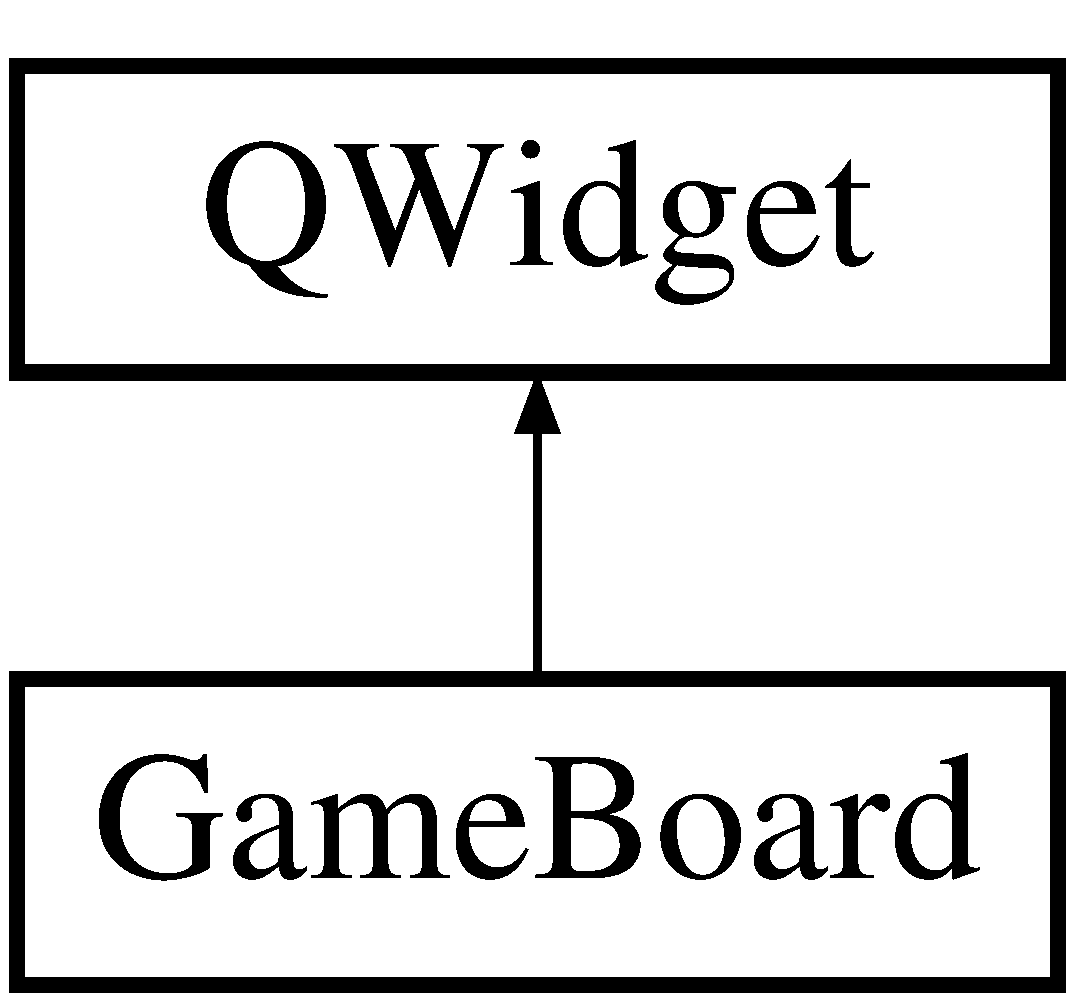
\includegraphics[height=2.000000cm]{class_game_board}
\end{center}
\end{figure}
\subsection*{Public Slots}
\begin{DoxyCompactItemize}
\item 
void \hyperlink{class_game_board_ae3c962a1819154c9f92910f1010019d3}{update\+Fs} ()
\begin{DoxyCompactList}\small\item\em It updates the location of the F\textquotesingle{}s. \end{DoxyCompactList}\end{DoxyCompactItemize}
\subsection*{Signals}
\begin{DoxyCompactItemize}
\item 
\hypertarget{class_game_board_a82c080b6518e1cf7753e71785c3afdcf}{}void {\bfseries game\+\_\+over} ()\label{class_game_board_a82c080b6518e1cf7753e71785c3afdcf}

\end{DoxyCompactItemize}
\subsection*{Public Member Functions}
\begin{DoxyCompactItemize}
\item 
\hyperlink{class_game_board_a02e83c0384303c16e8155ca759b882d0}{Game\+Board} (Q\+Widget $\ast$parent=0, size\+\_\+t board\+\_\+size=10, size\+\_\+t f\+\_\+speed=10, size\+\_\+t number\+\_\+of\+\_\+fs=1)
\begin{DoxyCompactList}\small\item\em \hyperlink{class_game_board}{Game\+Board} constructor. \end{DoxyCompactList}\item 
\hyperlink{class_game_board_a48e19b4953c87cc5eea1f9152d09499e}{$\sim$\+Game\+Board} ()
\begin{DoxyCompactList}\small\item\em \hyperlink{class_game_board_a48e19b4953c87cc5eea1f9152d09499e}{Game\+Board\+::$\sim$\+Game\+Board}. \end{DoxyCompactList}\item 
void \hyperlink{class_game_board_a3fdf1e6bfcc24a0930196be5fc3150c1}{key\+Press\+Event} (Q\+Key\+Event $\ast$event)
\begin{DoxyCompactList}\small\item\em \hyperlink{class_game_board_a3fdf1e6bfcc24a0930196be5fc3150c1}{Game\+Board\+::key\+Press\+Event}. \end{DoxyCompactList}\item 
void \hyperlink{class_game_board_a07896dc68fa3dc7ab7206e20da4c8dea}{paint\+Event} (Q\+Paint\+Event $\ast$e)
\begin{DoxyCompactList}\small\item\em \hyperlink{class_game_board_a07896dc68fa3dc7ab7206e20da4c8dea}{Game\+Board\+::paint\+Event}. \end{DoxyCompactList}\item 
void \hyperlink{class_game_board_a8cf0f1726da9d4fdfe9d044d290aca9d}{show\+Event} (Q\+Show\+Event $\ast$e)
\begin{DoxyCompactList}\small\item\em \hyperlink{class_game_board_a8cf0f1726da9d4fdfe9d044d290aca9d}{Game\+Board\+::show\+Event}. \end{DoxyCompactList}\item 
void \hyperlink{class_game_board_ad0652bc1afe57f5c90363ff23b085f1d}{munch\+Grade} (int x, int y)
\begin{DoxyCompactList}\small\item\em \hyperlink{class_game_board_ad0652bc1afe57f5c90363ff23b085f1d}{Game\+Board\+::munch\+Grade}. \end{DoxyCompactList}\item 
void \hyperlink{class_game_board_a41ac6cca98e3f787414574d1aeaac2d0}{update\+Student} (int px, int py, int nx, int ny)
\begin{DoxyCompactList}\small\item\em \hyperlink{class_game_board_a41ac6cca98e3f787414574d1aeaac2d0}{Game\+Board\+::update\+Student}. \end{DoxyCompactList}\item 
void \hyperlink{class_game_board_a705640e76fa5aaad98b40eec1a9ad9b1}{update\+After\+Munch} (bool flag)
\begin{DoxyCompactList}\small\item\em \hyperlink{class_game_board_a705640e76fa5aaad98b40eec1a9ad9b1}{Game\+Board\+::update\+After\+Munch}. \end{DoxyCompactList}\item 
\hypertarget{class_game_board_a68897815653f92727fff6cba9e07109b}{}bool {\bfseries is\+Valid\+Munch} (int x, int y)\label{class_game_board_a68897815653f92727fff6cba9e07109b}

\item 
\hypertarget{class_game_board_a2003859542d5189c632c4ec02feab6a1}{}int {\bfseries get\+Student\+Score} ()\label{class_game_board_a2003859542d5189c632c4ec02feab6a1}

\end{DoxyCompactItemize}


\subsection{Detailed Description}
class that creates a game board. 

it creates a game board where the user could move around the board and munch letter grades.. 

\subsection{Constructor \& Destructor Documentation}
\hypertarget{class_game_board_a02e83c0384303c16e8155ca759b882d0}{}\index{Game\+Board@{Game\+Board}!Game\+Board@{Game\+Board}}
\index{Game\+Board@{Game\+Board}!Game\+Board@{Game\+Board}}
\subsubsection[{Game\+Board}]{\setlength{\rightskip}{0pt plus 5cm}Game\+Board\+::\+Game\+Board (
\begin{DoxyParamCaption}
\item[{Q\+Widget $\ast$}]{parent = {\ttfamily 0}, }
\item[{size\+\_\+t}]{board\+\_\+sz = {\ttfamily 10}, }
\item[{size\+\_\+t}]{f\+\_\+spd = {\ttfamily 10}, }
\item[{size\+\_\+t}]{num\+\_\+of\+\_\+f = {\ttfamily 1}}
\end{DoxyParamCaption}
)\hspace{0.3cm}{\ttfamily [explicit]}}\label{class_game_board_a02e83c0384303c16e8155ca759b882d0}


\hyperlink{class_game_board}{Game\+Board} constructor. 

This constructs the board for the game. 
\begin{DoxyParams}{Parameters}
{\em parent} & is the widget on which the board will be created. \\
\hline
{\em board\+\_\+sz} & is the size of the board. \\
\hline
{\em f\+\_\+spd} & is the speed at which the grade letter F will be moving accross the board. \\
\hline
\end{DoxyParams}
\hypertarget{class_game_board_a48e19b4953c87cc5eea1f9152d09499e}{}\index{Game\+Board@{Game\+Board}!````~Game\+Board@{$\sim$\+Game\+Board}}
\index{````~Game\+Board@{$\sim$\+Game\+Board}!Game\+Board@{Game\+Board}}
\subsubsection[{$\sim$\+Game\+Board}]{\setlength{\rightskip}{0pt plus 5cm}Game\+Board\+::$\sim$\+Game\+Board (
\begin{DoxyParamCaption}
{}
\end{DoxyParamCaption}
)}\label{class_game_board_a48e19b4953c87cc5eea1f9152d09499e}


\hyperlink{class_game_board_a48e19b4953c87cc5eea1f9152d09499e}{Game\+Board\+::$\sim$\+Game\+Board}. 

\hyperlink{class_game_board}{Game\+Board} deconstructor-\/ it deallocates the memory that was used. 

\subsection{Member Function Documentation}
\hypertarget{class_game_board_a3fdf1e6bfcc24a0930196be5fc3150c1}{}\index{Game\+Board@{Game\+Board}!key\+Press\+Event@{key\+Press\+Event}}
\index{key\+Press\+Event@{key\+Press\+Event}!Game\+Board@{Game\+Board}}
\subsubsection[{key\+Press\+Event}]{\setlength{\rightskip}{0pt plus 5cm}void Game\+Board\+::key\+Press\+Event (
\begin{DoxyParamCaption}
\item[{Q\+Key\+Event $\ast$}]{event}
\end{DoxyParamCaption}
)}\label{class_game_board_a3fdf1e6bfcc24a0930196be5fc3150c1}


\hyperlink{class_game_board_a3fdf1e6bfcc24a0930196be5fc3150c1}{Game\+Board\+::key\+Press\+Event}. 

It identifies if the left,right,up,down, or spacebar keys were pressed and calls the update\+Student and munch\+Grade function. 
\begin{DoxyParams}{Parameters}
{\em event} & records the key from the keyboard that was pressed. \\
\hline
\end{DoxyParams}
\hypertarget{class_game_board_ad0652bc1afe57f5c90363ff23b085f1d}{}\index{Game\+Board@{Game\+Board}!munch\+Grade@{munch\+Grade}}
\index{munch\+Grade@{munch\+Grade}!Game\+Board@{Game\+Board}}
\subsubsection[{munch\+Grade}]{\setlength{\rightskip}{0pt plus 5cm}void Game\+Board\+::munch\+Grade (
\begin{DoxyParamCaption}
\item[{int}]{x, }
\item[{int}]{y}
\end{DoxyParamCaption}
)}\label{class_game_board_ad0652bc1afe57f5c90363ff23b085f1d}


\hyperlink{class_game_board_ad0652bc1afe57f5c90363ff23b085f1d}{Game\+Board\+::munch\+Grade}. 

It allows the student to munch the letter grade on the board. 
\begin{DoxyParams}{Parameters}
{\em x} & is the x-\/coordinate \\
\hline
{\em y} & is the y-\/coordinate \\
\hline
\end{DoxyParams}
\hypertarget{class_game_board_a07896dc68fa3dc7ab7206e20da4c8dea}{}\index{Game\+Board@{Game\+Board}!paint\+Event@{paint\+Event}}
\index{paint\+Event@{paint\+Event}!Game\+Board@{Game\+Board}}
\subsubsection[{paint\+Event}]{\setlength{\rightskip}{0pt plus 5cm}void Game\+Board\+::paint\+Event (
\begin{DoxyParamCaption}
\item[{Q\+Paint\+Event $\ast$}]{e}
\end{DoxyParamCaption}
)}\label{class_game_board_a07896dc68fa3dc7ab7206e20da4c8dea}


\hyperlink{class_game_board_a07896dc68fa3dc7ab7206e20da4c8dea}{Game\+Board\+::paint\+Event}. 

It sets the images(student and letter F) on their respective(current) location on the board. 
\begin{DoxyParams}{Parameters}
{\em e} & \\
\hline
\end{DoxyParams}
\hypertarget{class_game_board_a8cf0f1726da9d4fdfe9d044d290aca9d}{}\index{Game\+Board@{Game\+Board}!show\+Event@{show\+Event}}
\index{show\+Event@{show\+Event}!Game\+Board@{Game\+Board}}
\subsubsection[{show\+Event}]{\setlength{\rightskip}{0pt plus 5cm}void Game\+Board\+::show\+Event (
\begin{DoxyParamCaption}
\item[{Q\+Show\+Event $\ast$}]{e}
\end{DoxyParamCaption}
)}\label{class_game_board_a8cf0f1726da9d4fdfe9d044d290aca9d}


\hyperlink{class_game_board_a8cf0f1726da9d4fdfe9d044d290aca9d}{Game\+Board\+::show\+Event}. 

Sets the board as the main/active window and displays it 
\begin{DoxyParams}{Parameters}
{\em e} & \\
\hline
\end{DoxyParams}
\hypertarget{class_game_board_a705640e76fa5aaad98b40eec1a9ad9b1}{}\index{Game\+Board@{Game\+Board}!update\+After\+Munch@{update\+After\+Munch}}
\index{update\+After\+Munch@{update\+After\+Munch}!Game\+Board@{Game\+Board}}
\subsubsection[{update\+After\+Munch}]{\setlength{\rightskip}{0pt plus 5cm}void Game\+Board\+::update\+After\+Munch (
\begin{DoxyParamCaption}
\item[{bool}]{flag}
\end{DoxyParamCaption}
)}\label{class_game_board_a705640e76fa5aaad98b40eec1a9ad9b1}


\hyperlink{class_game_board_a705640e76fa5aaad98b40eec1a9ad9b1}{Game\+Board\+::update\+After\+Munch}. 

It updates the 
\begin{DoxyParams}{Parameters}
{\em flag} & will determine \\
\hline
\end{DoxyParams}
\hypertarget{class_game_board_ae3c962a1819154c9f92910f1010019d3}{}\index{Game\+Board@{Game\+Board}!update\+Fs@{update\+Fs}}
\index{update\+Fs@{update\+Fs}!Game\+Board@{Game\+Board}}
\subsubsection[{update\+Fs}]{\setlength{\rightskip}{0pt plus 5cm}void Game\+Board\+::update\+Fs (
\begin{DoxyParamCaption}
{}
\end{DoxyParamCaption}
)\hspace{0.3cm}{\ttfamily [slot]}}\label{class_game_board_ae3c962a1819154c9f92910f1010019d3}


It updates the location of the F\textquotesingle{}s. 

It randomly updates the location of the F\textquotesingle{}s around the game board. \hypertarget{class_game_board_a41ac6cca98e3f787414574d1aeaac2d0}{}\index{Game\+Board@{Game\+Board}!update\+Student@{update\+Student}}
\index{update\+Student@{update\+Student}!Game\+Board@{Game\+Board}}
\subsubsection[{update\+Student}]{\setlength{\rightskip}{0pt plus 5cm}void Game\+Board\+::update\+Student (
\begin{DoxyParamCaption}
\item[{int}]{px, }
\item[{int}]{py, }
\item[{int}]{nx, }
\item[{int}]{ny}
\end{DoxyParamCaption}
)}\label{class_game_board_a41ac6cca98e3f787414574d1aeaac2d0}


\hyperlink{class_game_board_a41ac6cca98e3f787414574d1aeaac2d0}{Game\+Board\+::update\+Student}. 

It updates the position of the student on the board. 
\begin{DoxyParams}{Parameters}
{\em px} & is the previous x-\/coordinate of the student\textquotesingle{}s location on the board. \\
\hline
{\em py} & is the previous y-\/coordinate of the student\textquotesingle{}s location on the board. \\
\hline
{\em nx} & is the new x-\/coordinate of the student\textquotesingle{}s location on the board. \\
\hline
{\em ny} & is the new y-\/coordinate of the student\textquotesingle{}s location on the board. \\
\hline
\end{DoxyParams}


The documentation for this class was generated from the following files\+:\begin{DoxyCompactItemize}
\item 
gameboard.\+h\item 
gameboard.\+cpp\end{DoxyCompactItemize}

\hypertarget{class_main_window}{}\section{Main\+Window Class Reference}
\label{class_main_window}\index{Main\+Window@{Main\+Window}}


class for the main window of game  




{\ttfamily \#include $<$mainwindow.\+h$>$}

Inheritance diagram for Main\+Window\+:\begin{figure}[H]
\begin{center}
\leavevmode
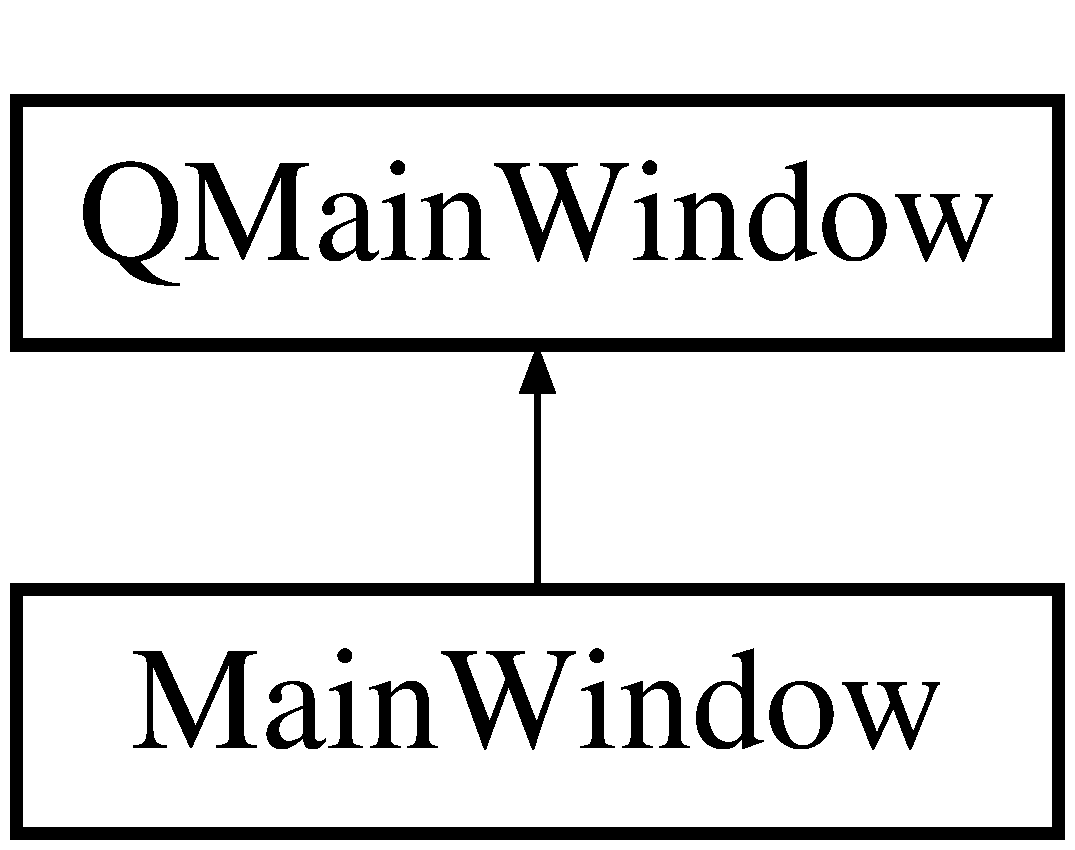
\includegraphics[height=2.000000cm]{class_main_window}
\end{center}
\end{figure}
\subsection*{Public Slots}
\begin{DoxyCompactItemize}
\item 
\hypertarget{class_main_window_a8cb2a71b4571b250bba40178f58b065c}{}void \hyperlink{class_main_window_a8cb2a71b4571b250bba40178f58b065c}{easy\+\_\+game\+\_\+begin} ()\label{class_main_window_a8cb2a71b4571b250bba40178f58b065c}

\begin{DoxyCompactList}\small\item\em It starts the game on easy mode. \end{DoxyCompactList}\item 
void \hyperlink{class_main_window_afefe9454f7bc872888ce48c4efbdc926}{medium\+\_\+game\+\_\+begin} ()
\begin{DoxyCompactList}\small\item\em It starts the game on medium mode. \end{DoxyCompactList}\item 
\hypertarget{class_main_window_a11aed9109e49c6ea802ff6cdd081fb76}{}void \hyperlink{class_main_window_a11aed9109e49c6ea802ff6cdd081fb76}{hard\+\_\+game\+\_\+begin} ()\label{class_main_window_a11aed9109e49c6ea802ff6cdd081fb76}

\begin{DoxyCompactList}\small\item\em It starts the game on hard mode. \end{DoxyCompactList}\item 
void \hyperlink{class_main_window_a6ccf59c9c1c8d6da887106200e675519}{game\+\_\+play} ()
\begin{DoxyCompactList}\small\item\em It provides the user with instructions. \end{DoxyCompactList}\item 
\hypertarget{class_main_window_ad095804e948ea80ebaa1311858700ded}{}void \hyperlink{class_main_window_ad095804e948ea80ebaa1311858700ded}{game\+\_\+over} ()\label{class_main_window_ad095804e948ea80ebaa1311858700ded}

\begin{DoxyCompactList}\small\item\em It ends and exits the game. \end{DoxyCompactList}\end{DoxyCompactItemize}
\subsection*{Public Member Functions}
\begin{DoxyCompactItemize}
\item 
\hyperlink{class_main_window_a8b244be8b7b7db1b08de2a2acb9409db}{Main\+Window} (Q\+Widget $\ast$parent=0)
\begin{DoxyCompactList}\small\item\em \hyperlink{class_main_window_a8b244be8b7b7db1b08de2a2acb9409db}{Main\+Window\+::\+Main\+Window} constructor. \end{DoxyCompactList}\item 
\hypertarget{class_main_window_ae98d00a93bc118200eeef9f9bba1dba7}{}\hyperlink{class_main_window_ae98d00a93bc118200eeef9f9bba1dba7}{$\sim$\+Main\+Window} ()\label{class_main_window_ae98d00a93bc118200eeef9f9bba1dba7}

\begin{DoxyCompactList}\small\item\em deconstructor of the \hyperlink{class_main_window}{Main\+Window} \end{DoxyCompactList}\end{DoxyCompactItemize}


\subsection{Detailed Description}
class for the main window of game 

it displays buttons to select the level of game play. 

\subsection{Constructor \& Destructor Documentation}
\hypertarget{class_main_window_a8b244be8b7b7db1b08de2a2acb9409db}{}\index{Main\+Window@{Main\+Window}!Main\+Window@{Main\+Window}}
\index{Main\+Window@{Main\+Window}!Main\+Window@{Main\+Window}}
\subsubsection[{Main\+Window}]{\setlength{\rightskip}{0pt plus 5cm}Main\+Window\+::\+Main\+Window (
\begin{DoxyParamCaption}
\item[{Q\+Widget $\ast$}]{parent = {\ttfamily 0}}
\end{DoxyParamCaption}
)\hspace{0.3cm}{\ttfamily [explicit]}}\label{class_main_window_a8b244be8b7b7db1b08de2a2acb9409db}


\hyperlink{class_main_window_a8b244be8b7b7db1b08de2a2acb9409db}{Main\+Window\+::\+Main\+Window} constructor. 

It creates the main window and displays it. 
\begin{DoxyParams}{Parameters}
{\em parent} & is the widget that will be passed to the main window to be displayed. \\
\hline
\end{DoxyParams}


\subsection{Member Function Documentation}
\hypertarget{class_main_window_a6ccf59c9c1c8d6da887106200e675519}{}\index{Main\+Window@{Main\+Window}!game\+\_\+play@{game\+\_\+play}}
\index{game\+\_\+play@{game\+\_\+play}!Main\+Window@{Main\+Window}}
\subsubsection[{game\+\_\+play}]{\setlength{\rightskip}{0pt plus 5cm}void Main\+Window\+::game\+\_\+play (
\begin{DoxyParamCaption}
{}
\end{DoxyParamCaption}
)\hspace{0.3cm}{\ttfamily [slot]}}\label{class_main_window_a6ccf59c9c1c8d6da887106200e675519}


It provides the user with instructions. 

It creates a new window with the game instructions. \hypertarget{class_main_window_afefe9454f7bc872888ce48c4efbdc926}{}\index{Main\+Window@{Main\+Window}!medium\+\_\+game\+\_\+begin@{medium\+\_\+game\+\_\+begin}}
\index{medium\+\_\+game\+\_\+begin@{medium\+\_\+game\+\_\+begin}!Main\+Window@{Main\+Window}}
\subsubsection[{medium\+\_\+game\+\_\+begin}]{\setlength{\rightskip}{0pt plus 5cm}void Main\+Window\+::medium\+\_\+game\+\_\+begin (
\begin{DoxyParamCaption}
{}
\end{DoxyParamCaption}
)\hspace{0.3cm}{\ttfamily [slot]}}\label{class_main_window_afefe9454f7bc872888ce48c4efbdc926}


It starts the game on medium mode. 


\begin{DoxyItemize}
\item 
\end{DoxyItemize}

The documentation for this class was generated from the following files\+:\begin{DoxyCompactItemize}
\item 
mainwindow.\+h\item 
mainwindow.\+cpp\end{DoxyCompactItemize}

%--- End generated contents ---

% Index
\backmatter
\newpage
\phantomsection
\clearemptydoublepage
\addcontentsline{toc}{chapter}{Index}
\printindex

\end{document}
